% !TeX spellcheck = en_US
%\documentclass[12pt]{article}

\documentclass[11pt]{report}

\usepackage[a4paper, margin=1in]{geometry}

\usepackage{mathtools}
\usepackage{footnote}
\usepackage{listings}
\usepackage{xcolor}
\usepackage{mathtools}
\usepackage{pdfpages}
\usepackage[english]{babel}
\usepackage[labelfont=bf]{caption}
\usepackage{float}
\captionsetup{labelfont=bf}
\usepackage[normalem]{ulem}

\useunder{\uline}{\ul}{}

\definecolor{codegreen}{rgb}{0,0.6,0}
\definecolor{codegray}{rgb}{0.5,0.5,0.5}
\definecolor{codepurple}{rgb}{0.58,0,0.82}
\definecolor{backcolour}{rgb}{0.95,0.95,0.95}
\usepackage{titlesec, color}

\definecolor{gray75}{gray}{0.75}
\newcommand{\hsp}{\hspace{10pt}}
%\titleformat{\section}[hang]{\Huge\bfseries}{\thesection\hsp\textcolor{gray75}{|}\hsp}{0pt}{\Huge\bfseries}

\lstdefinestyle{mystyle}{
	backgroundcolor=\color{backcolour},   
	commentstyle=\color{codegreen},
	keywordstyle=\color{blue},
	numberstyle=\tiny\color{codegray},
	stringstyle=\color{orange},
	basicstyle=\ttfamily\footnotesize,
	breakatwhitespace=false,         
	breaklines=true,                 
	captionpos=b,                    
	keepspaces=true,                 
	numbers=left,                    
	numbersep=5pt,                  
	showspaces=false,                
	showstringspaces=false,
	showtabs=false,                  
	tabsize=2
}

\lstset{style=mystyle}

\includeonly{
	chapters/introduction,
	chapters/modeling,
	chapters/implementation,
	chapters/verification,
	chapters/simulation_experiments,
	chapters/conclusions
}

\begin{document}


\begin{titlepage}
	\begin{center}
		\begin{figure}
			
\includegraphics[width=\textwidth]{img/marchio_unipi_pant541-eps-converted-to.pdf}         
		\end{figure}
		{\Large
			Computer Engineering\\
			\vspace{5mm} %5mm vertical space
			Foundations of Cybersecurity}\\
		\vspace{30mm} %5mm vertical space
		{\Huge\textbf{\textit{secureCom}}}\\
		\vspace{10mm} %5mm vertical space
		{\Large Group Project Report}\\
		\par\noindent\rule{\textwidth}{0.4pt}
		\begin{flushright}
			\textit{TEAM MEMBERS}:\\ 
			Francesco Iemma\\
			Yuri Mazzuoli\\ 
			Olgerti Xhanej\\
			
		\end{flushright}
		\vfill
		Academic Year: 2020/2021\\        
	\end{center}
\end{titlepage} 
\tableofcontents
\chapter{Specifications}
	\noindent The project consist on an application for secure communication between 2 clients through an intermediate server.
	\newline
	The server have to:
	\begin{itemize}
		\item authenticate clients on connecting to it (with pre-shared public key)
		\item authenticate ifself with a certificate
		\item provide the list of online clients
		\item relay messsages from one client to another, together with chat requests and response
		\item provide to a client the public key of another client, in order to permit a secure communication between them
	\end{itemize}
	A client have to:
	\begin{itemize}
		\item authenticate the server on connecting to it (with the certificate)
		\item authenticate himself with its public key
	\end{itemize}
	A client can:
	\begin{itemize}
		\item print the list of online clients
		\item authenticate another client via its public key obtained from the server
		\item request to chat with another client
		\item answer to a chat request (if not already involved in another chat)
		\item when in a chat, exchange text messages with another client or close the chat
	\end{itemize}

\newpage
\chapter{Design choises}
\section{Client Server Handshake}
In order to authenticate themselvse and enstablish a session key to securely communicate, a client
and the server have to exchange handshake messages. We implement this protocol to provide perfect 
forward secrecy, starting from the pre-shared cryptographic quantities (public keys and certificates):
\begin{figure}[H]
	\centering
	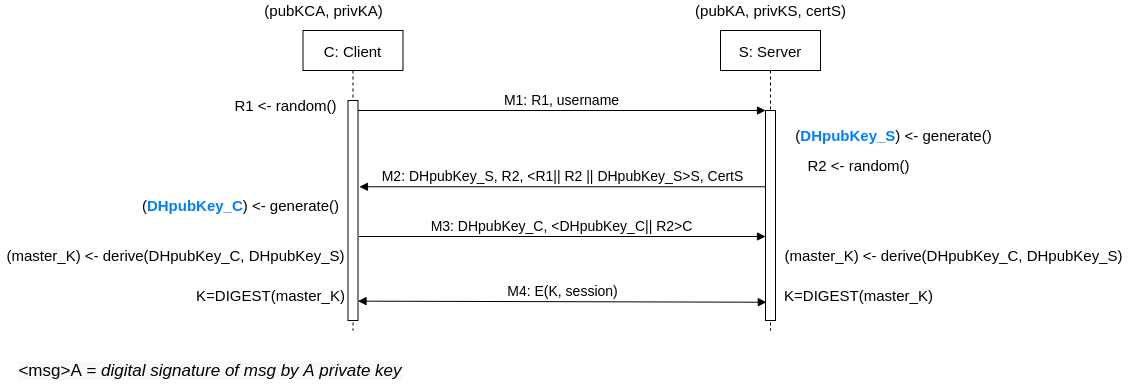
\includegraphics[scale=0.19]{img/AuthClientServer.png}
	\caption{Client Server Handshake Protocol Schema}
	\label {img: AuthClientServer}
\end{figure}
This handshake is a custom implementation of an ephimeral Diffie-Hellman Key Exchange, in which we ensure
protection against the man in the middle attack with random nuances (R1 and R2). The client is able to 
authenticate the server via it's certificate, signed by a trusted certification authority (the client
is distributed along with CA's self-signed certificate); the server have a built-in list of all client's
public keys. DH's private keys are deleted after the handshake and the key is generated by a digest of the 
shared seceret: in this way we provide security against a future disclousure of one of the long term private keys.

\newpage
\section{Chat Request}
With the client-server handshake we build a secure tunnel between each client and the server. Using this 
tunnel every client can execute command on the server in a secure way; the most important (and complex) command
is a chat request, of which we provide a scheme:
\begin{figure}[H]
	\centering
	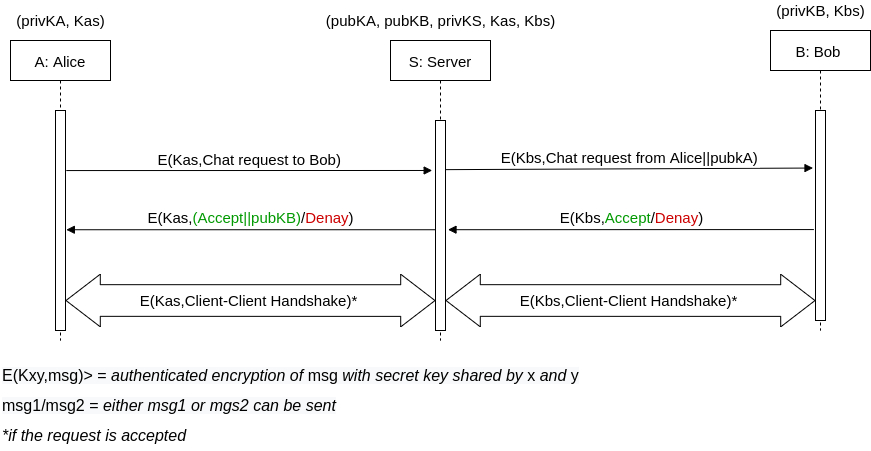
\includegraphics[scale=0.2]{img/ChatRequest.png}
	\caption{Chat Request Protocol Schema}
	\label {img: ChatRequest}
\end{figure}
The server is obliged to communicate correct public keys.
\section{Client to Client handshake}
In order to guarantee a secure communication of the clients agaist the server, we perform an ephimeral 
Diffie-Hellman Key Exchange befor starting the chat. In this case the two parties already know each other
public keys, because the server provided them. 
\begin{figure}[H]
	\centering
	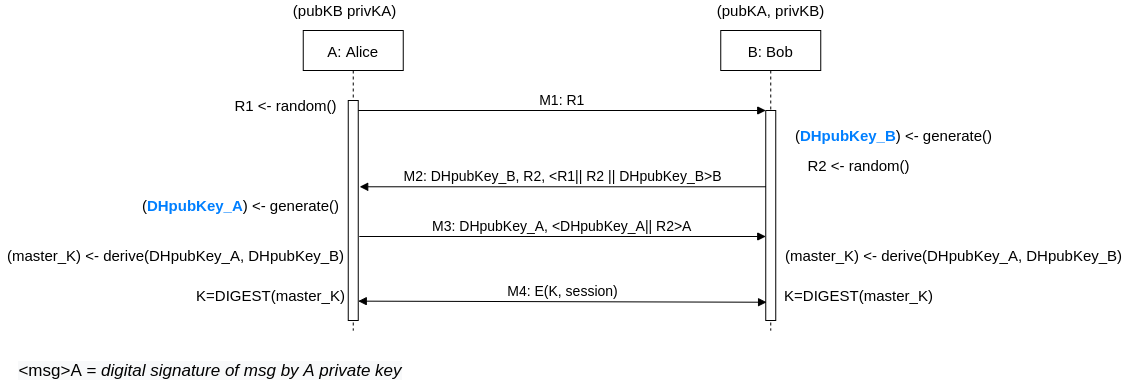
\includegraphics[scale=0.19]{img/AuthClientClient.png}
	\caption{Client Client Handshake Protocol Schema}
	\label {img: AuthClientClient}
\end{figure}
The server in not represented because it only retransmit messages from a client to the other without changing
anything; if the server try to implement a "man in the middle" attack he will only obtain a denial of service
because the protocol is protected by private key signatures. Also in this case, DH keys are discared after 
the handshake, and future messages are numbered againts reply attacks.



\chapter{Implemetation}
\section{Software Architecture}
From an implementation prospective, the client program has to communicate with user and server; in the
server program instead, messages have to pass from one process to another in order to be delivered to the
recipient client.
\begin{figure}[H]
	\centering
	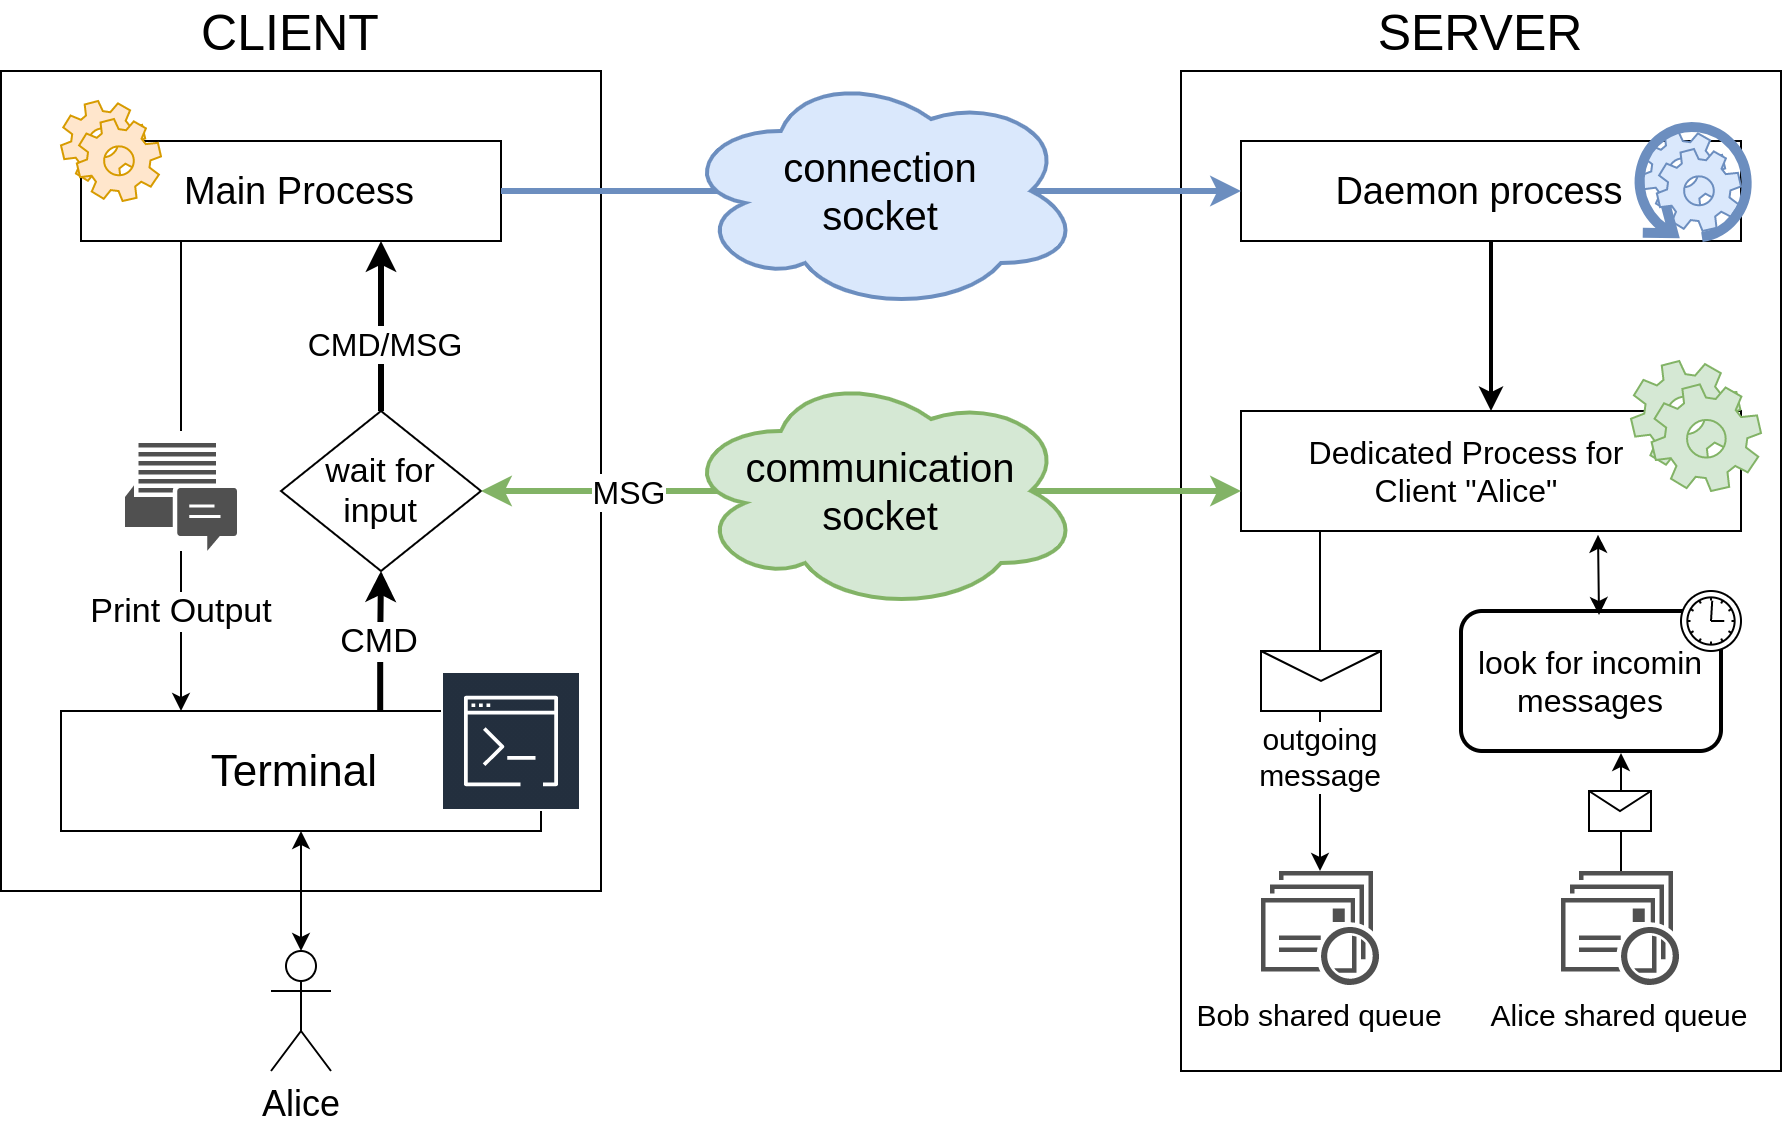
\includegraphics[scale=0.24]{img/Implementation_scheme.png}
	\caption{Implementation scheme}
	\label {img: Implementation_scheme}
\end{figure}
At the beginning the client will connect to a standard server port which is in listening state; than the communication
is commuted to another port, with a dedicated server process. At the end of the secure handshake, the process will be 
dedicated to the authenticated user who is connected. This server process is able to read from his dedicated queue of 
incoming messages, and relay messages to others client via their queue; at constant intervals a timer will read all the 
messages from the incomin queue and it will forward them to the client. When this behaveour is unwanted, the relative interrupt
is disabled.
Using the system call \texttt{select()} the client is able to listen from multiple source of input, in this
case communication socket and terminal. In this way the client program is able, for example, to automatically refuse a chat request 
when the user is already chatting.

\section{Alghoritms and Protocols}
We briefly describe the cypher suite we choose to use in order to guarantee security specifications.
Cyphers are the same for Cient-Server and Cient-Cient communication, specific message formats are reported In
Capter 4.
\subsection{Public Key Authentication}
\paragraph*{Long Term Keys}
The Cerification Authority (CA) have a \texttt{Publick Key}, included in a self-signed
certificate; the corresponding private key is embedded in the program for certificate generation, 
SimpleAuthority \footnote{https://simpleauthority.com}.
CA's cerficiate and Revocation List (CRL) are exported and distributed with client executable.
The server cerfificate, which is signed by CA, contains the \texttt{Publick Key} of the server; it
is stored server side, and provided to the client during the handshake.
Clients Public Keys are also stored in the server, while only the client hold its Private Key.
All keys are \texttt{RSA Key Pairs with 2048-bits Public Keys} and are stored in \texttt{.pem} format, as certificates and CRLs are.
\paragraph*{Short Term Keys}
Handshakes protocols are performed with the Ephimeral Diffie-Hellman Key Exchange. 
We choose to use the Elliptic Curve implenetation because is very efficent (in term of performance vs security strenght);
we use \verb|NID_X9_62_prime256v1| standard parameters that ensure 128-bits secuiry strenght with a 256-bits curve. We use the \texttt{SHA-256} digest of the \texttt{shared secret} as
the session key.
To ensure freshness in the challenge-response scheme we use \texttt{16 bytes nonces}.
\subsection{Authenticated Encryption}
From the handshake we obtain a 256-bits simmetric key which is used in \texttt{AES-256 GCM} authenticated encryprion protocol.
We use a \texttt{16 bytes} tag for authentication of cyphertext and clear fields in the header. GCM scheme ensure a cyphertext
size equal to the plaintext size; this makes programming easier, mantaining an optimal resistance against all known attacks.
Messages exchanged in sessions are numbered, starting from 1, to a maximum of $2^{32}-1$ (\verb|0xFFFFFFFF|), which is the
maximum integer representable on 32 bits; this will make possible to identify a message reply, done
my an attacker. The session is automatically closed when a message with number \verb|0xFFFFFFFF| is recived.
Clients mantains two counter for the communication with the server:  one for the next message to send and another for
the next message to receive; the same thing is done for the communication with another client (to prevent the server to 
reply a message); also the server has to implement this behaveour in sessions with clients.

\subsection*{Note on Chat message encryprion }
Chat message are encrypted twice, one time with the and Cient-Cient session key and 
the second one with Cient-Server session key; this will not double the BIT strenght of the cypher against 
a brute force attack, because of the \texttt{meet in the middle} attack. 
At the same time, this fact makes the system more secure agaist a password recover attack; in case, for
whatever reason, a session key between clients is discover by an attacker, this will not be enaugh for read private messages,
because the attacker have to discover also the session key between a client and the server.

\chapter{Messages Format}

\section{Handshake}
\subsection*{Client Server Handshake}
\begin{figure}[H]
	\centering
	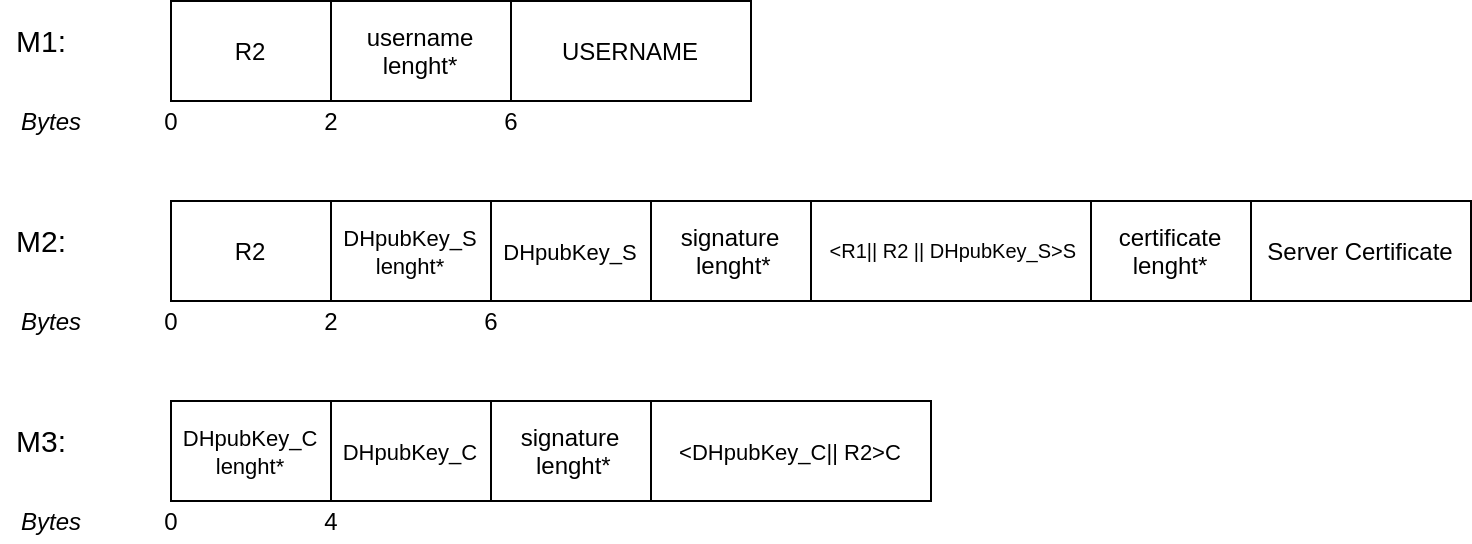
\includegraphics[scale=0.28]{img/AuthClientServer_messageFormat.png}
	\caption{Client Server Handshake Message Format}
	\label {img: FormatClientServer}
\end{figure}
\subsection*{Headers}
\begin{figure}[H]
	\centering
	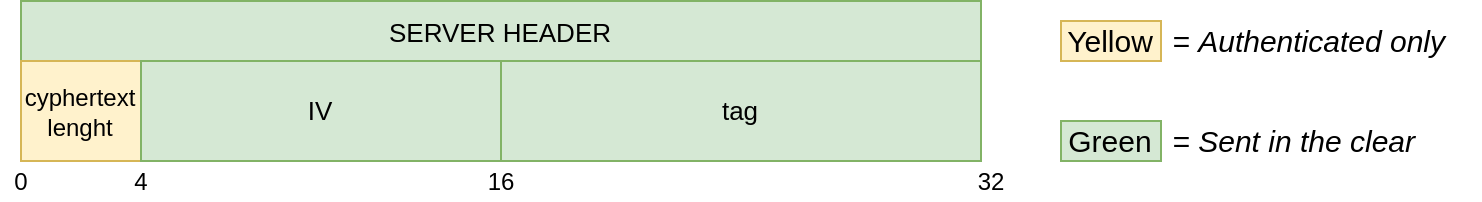
\includegraphics[scale=0.24]{img/HeaderFormat.png}
	\caption{Client Server Header Format}
	\label {img: FormatClientServerHeader}
\end{figure}
\subsection*{Client Client Handshake}
\begin{figure}[H]
	\centering
	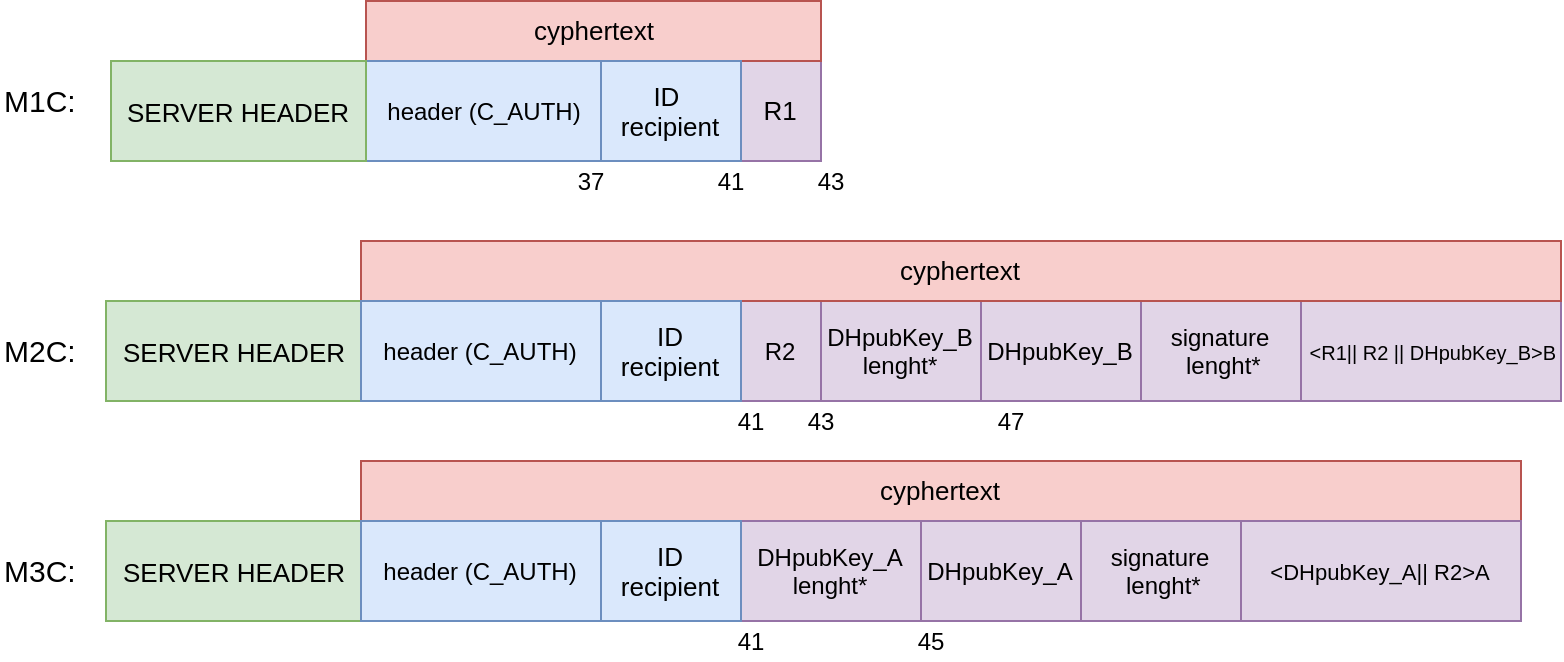
\includegraphics[scale=0.28]{img/AuthClientClient_messageFormat.png}
	\caption{Client Client Handshake Message Format}
	\label {img: FormatClientClient}
\end{figure}

\section{Commands}
\begin{figure}[H]
	\centering
	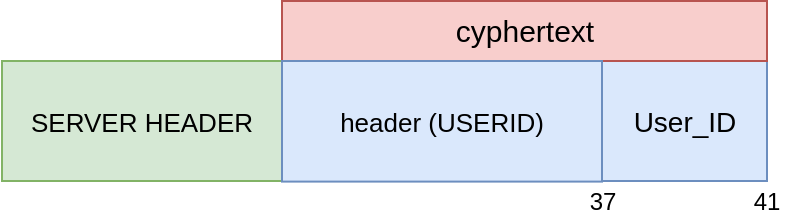
\includegraphics[scale=0.28]{img/SessionFirstMessageFormat.png}
	\caption{First message of every Session: server communicate cliet userID}
	\label {img: FormatClientServerFirst}
\end{figure}
\subsection*{Client Online List Request and Answer }
\begin{figure}[H]
	\centering
	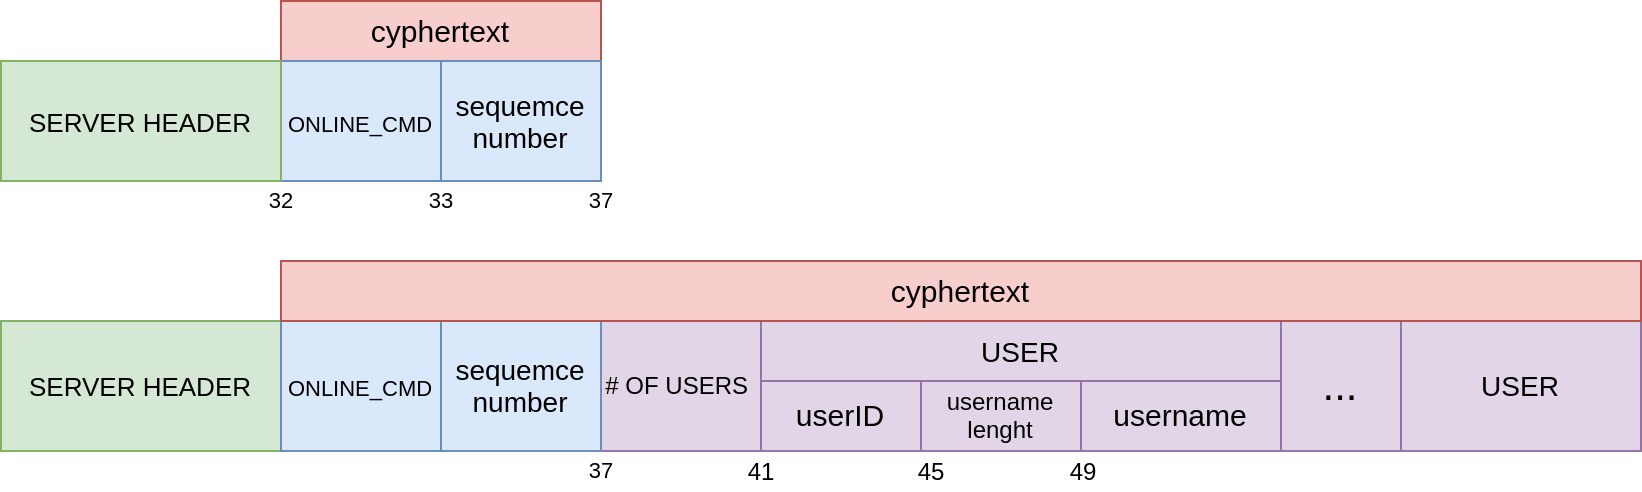
\includegraphics[scale=0.25]{img/ClientOnline_messageFormat.png}
	\caption{Client Online Message Format}
	\label {img: FormatClientOnline}
\end{figure}
\subsection*{Other commands}
\begin{figure}[H]
	\centering
	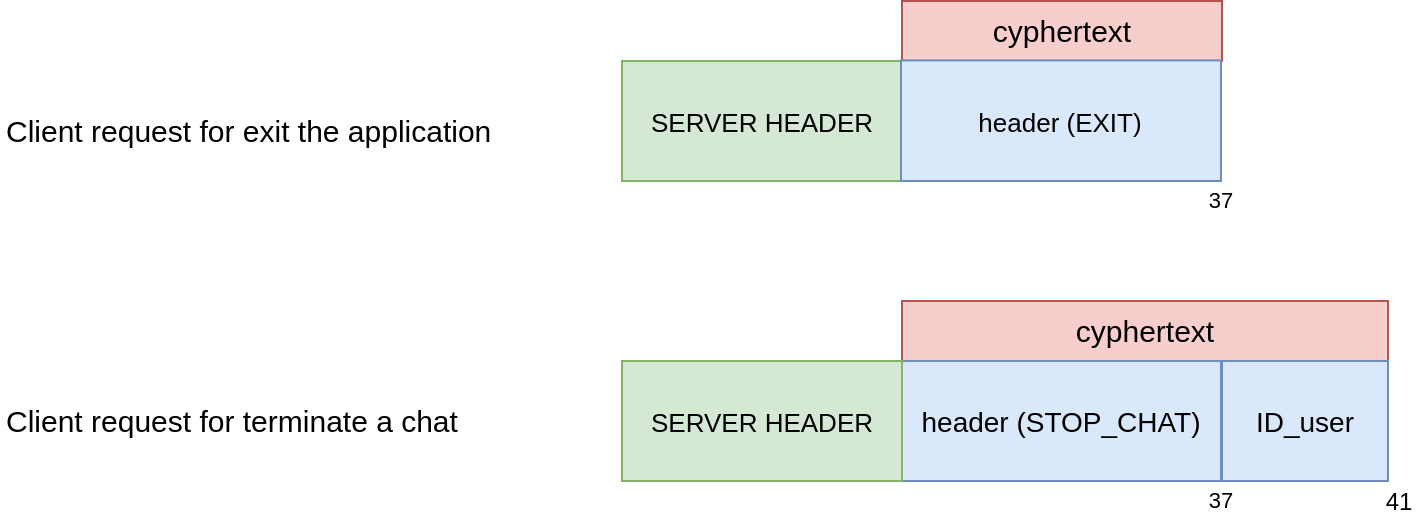
\includegraphics[scale=0.28]{img/OthersCommandsFormat.png}
	\caption{Other commands Format}
	\label {img: FormatOtherCommands}
\end{figure}
\subsection*{Chat Request and Answers}
\begin{figure}[H]
	\centering
	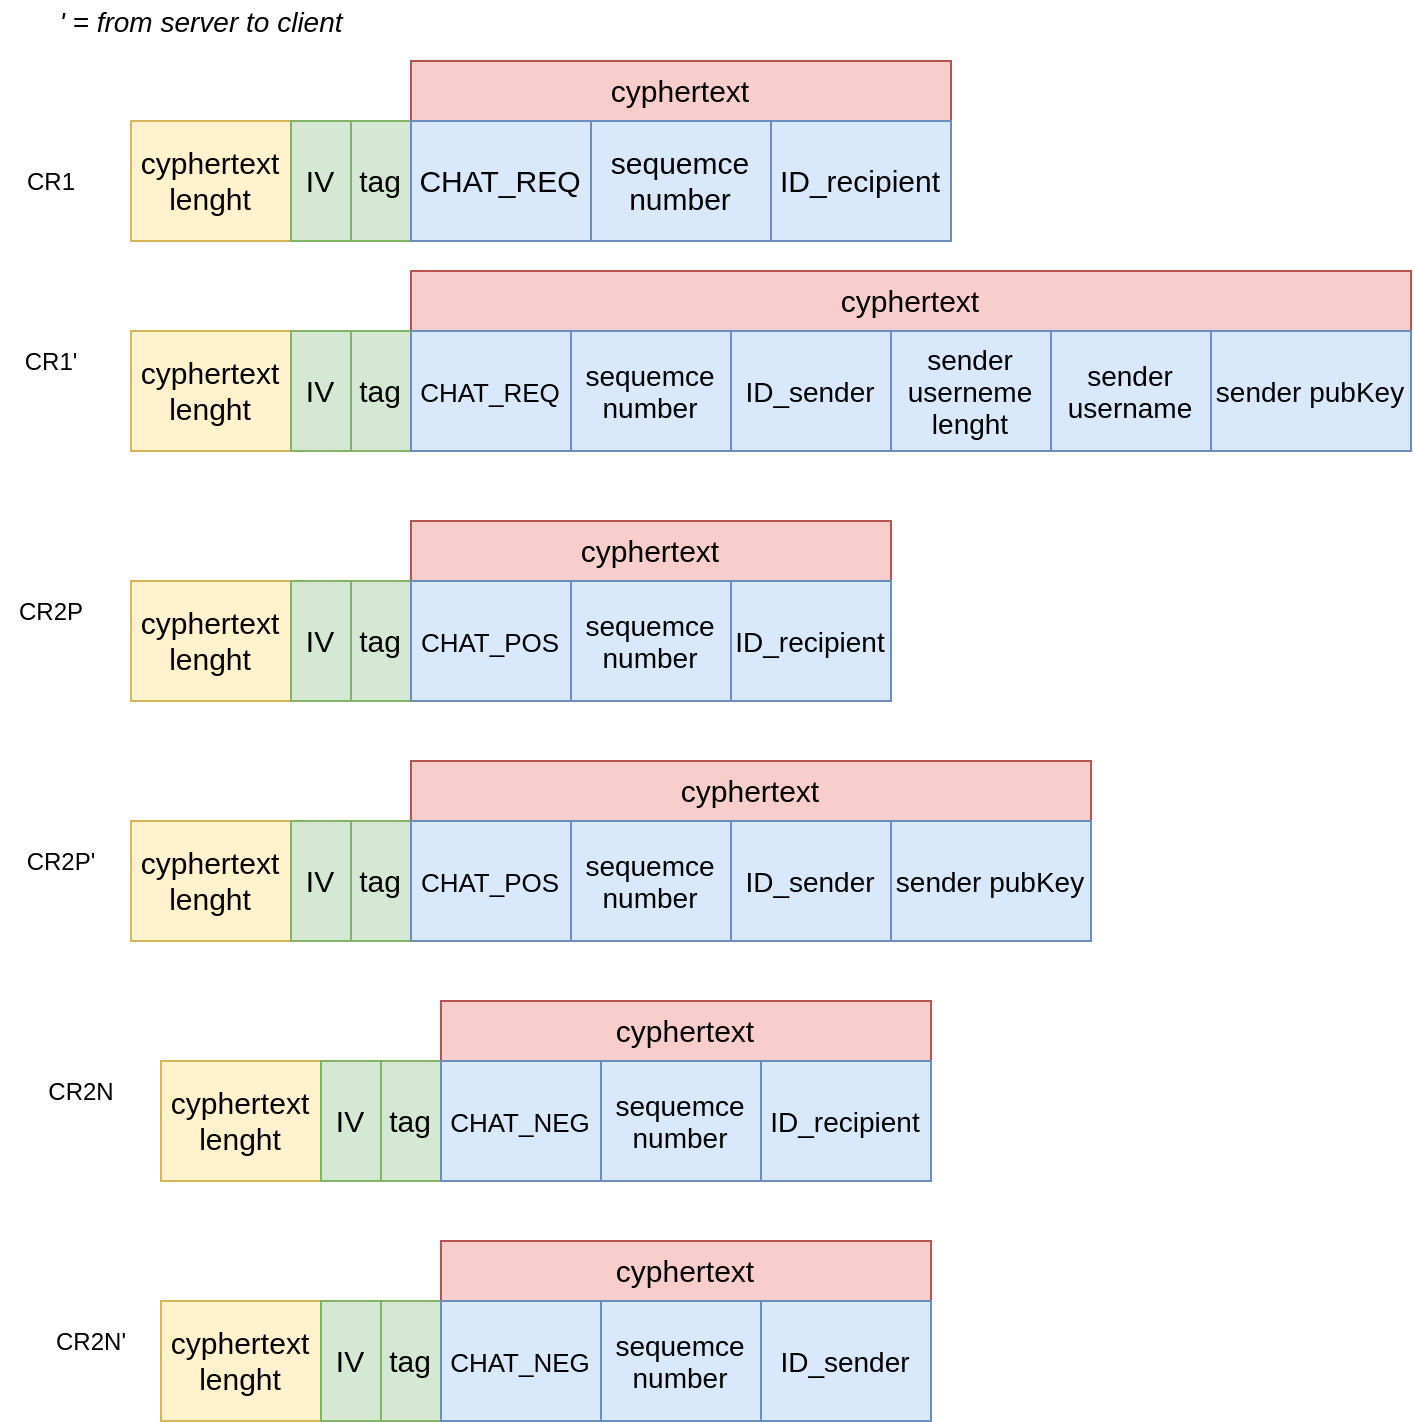
\includegraphics[scale=0.28]{img/ChatRequest_messageFormat.png}
	\caption{Chat Request Message Format}
	\label {img: FormatChatRequest}
\end{figure}
\newpage

\section{Chat}
\begin{figure}[H]
	\centering
	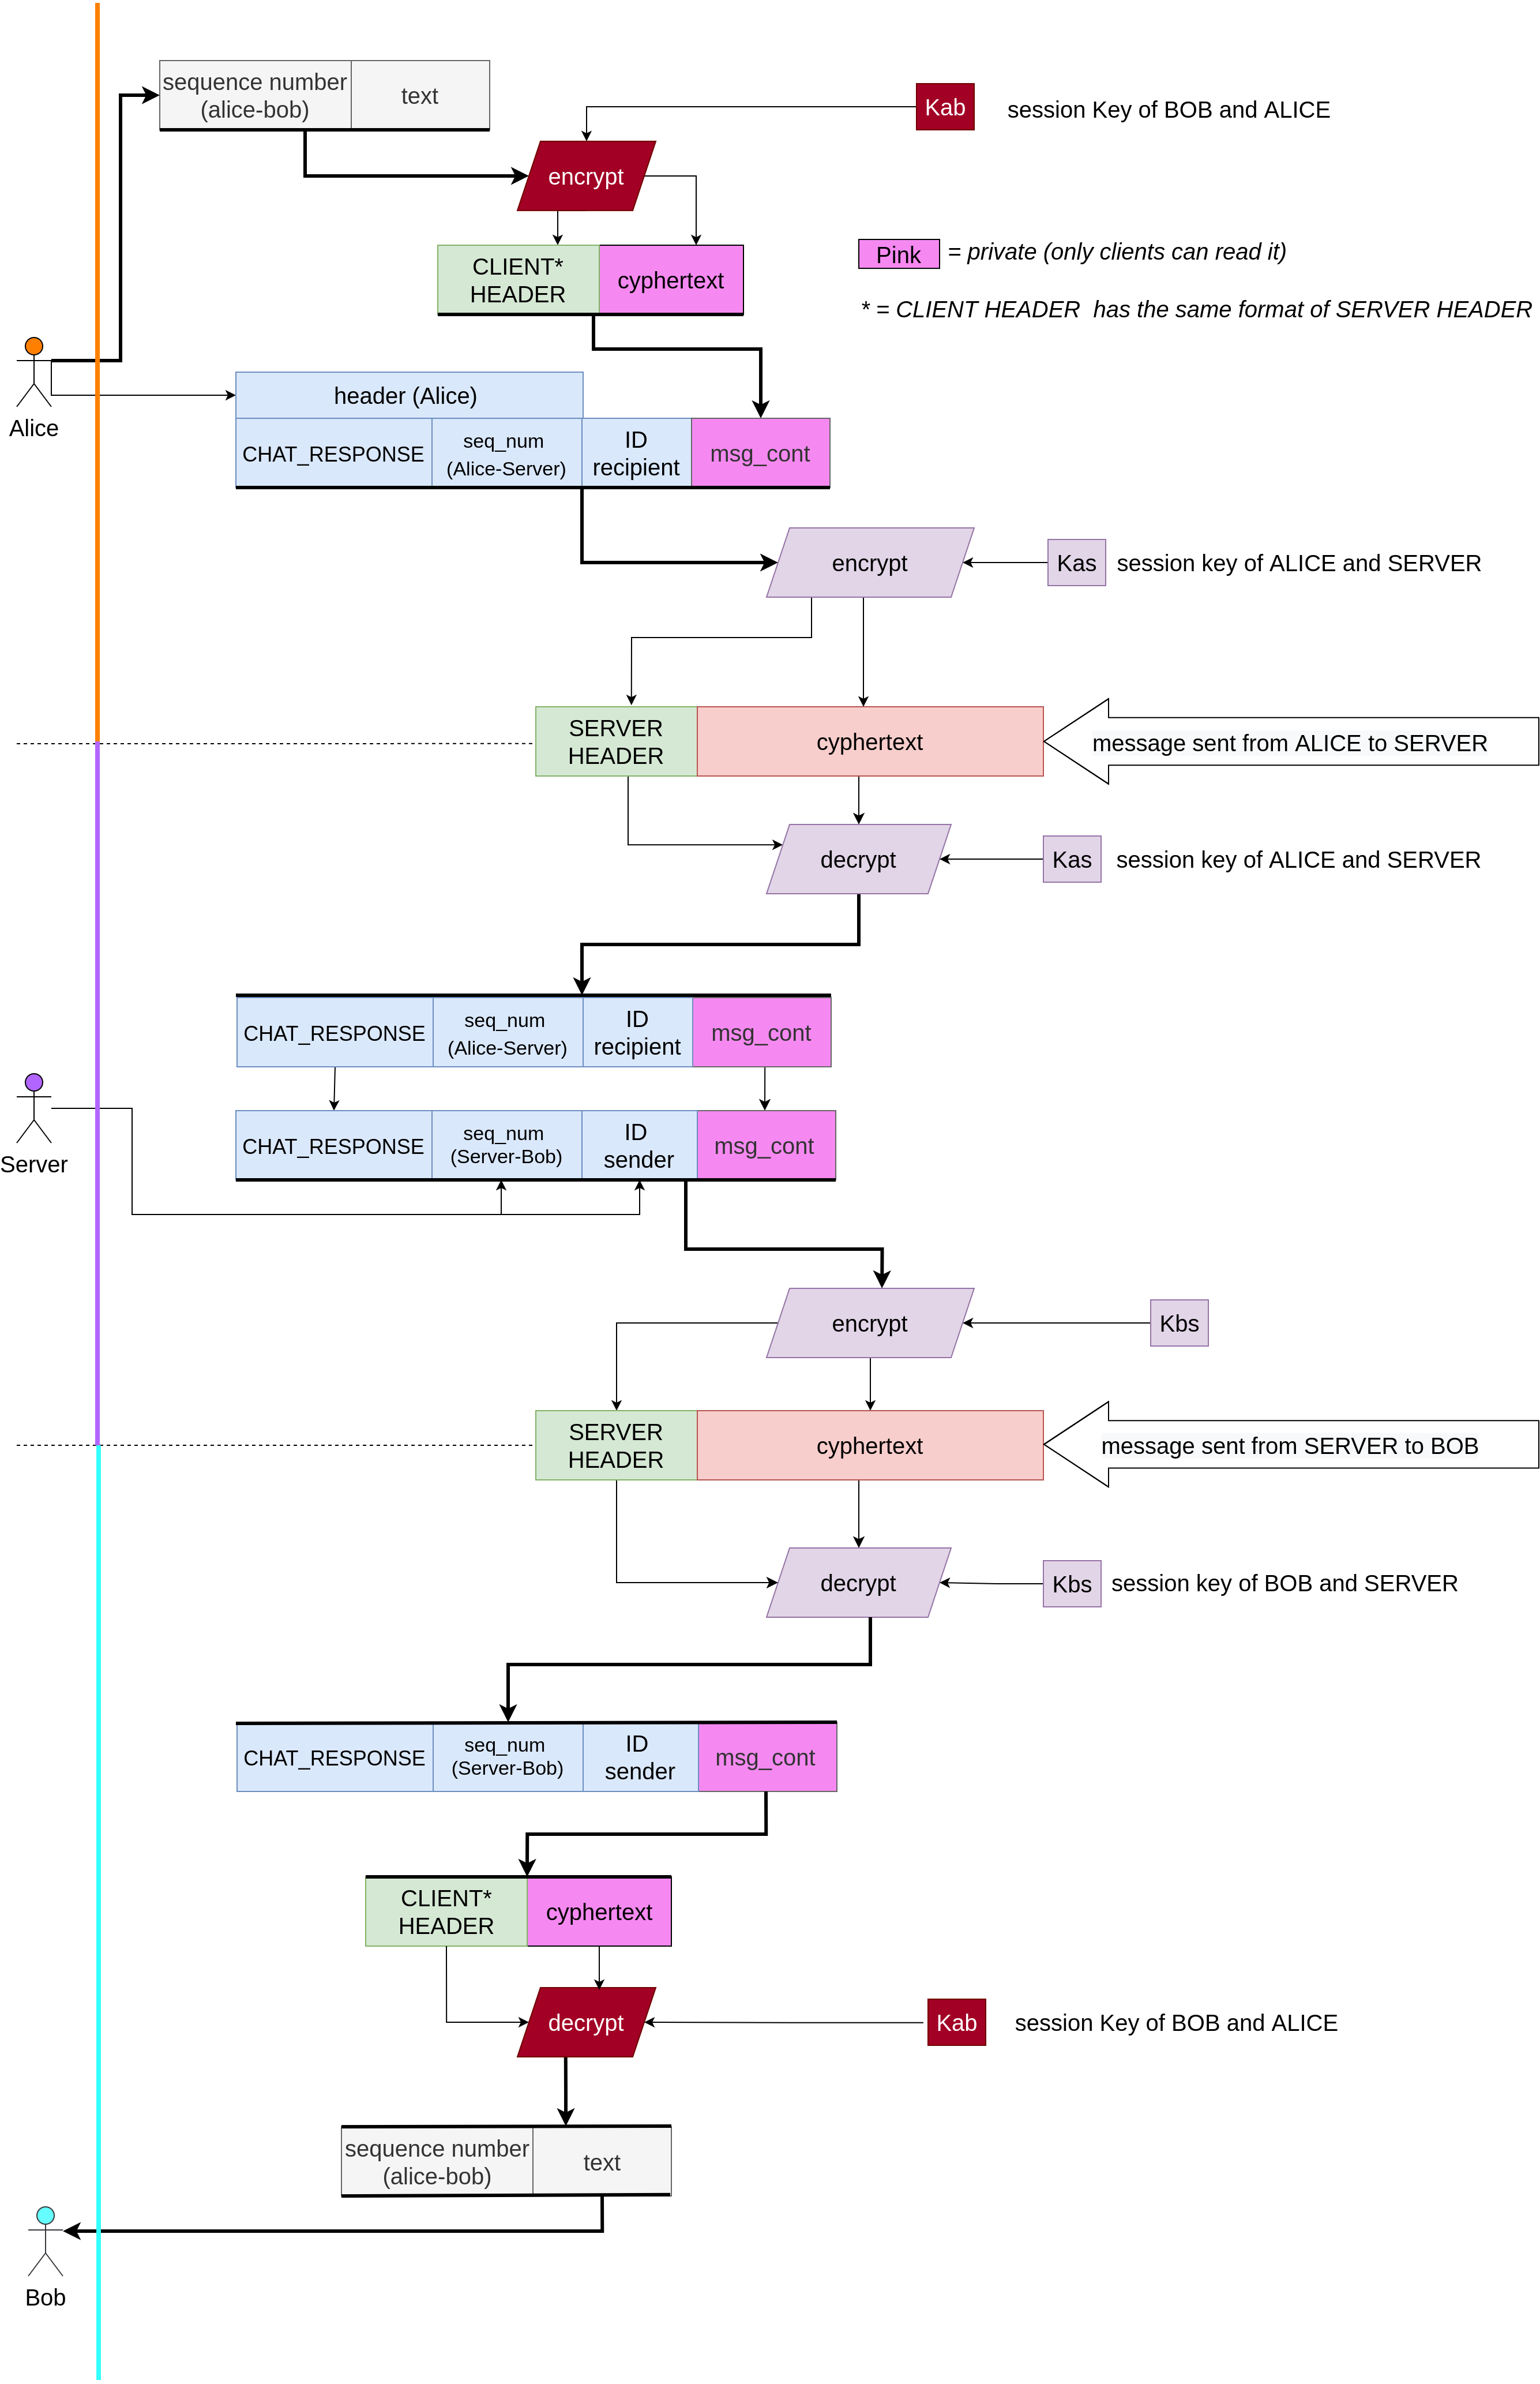
\includegraphics[scale=0.09]{img/message_relay.png}
	\caption{Client Client Handshake Protocol Schema}
	\label {img: MessageRelay}
\end{figure}



	
%	\item A third solution can be adding a command to indicate that a client is available to receive chat request. Thus:
	
%	\begin{enumerate}
%		\item A users is online when it has launched the command "available" (isChatting = false). Notice that in this case the variable isChatting can be called in a more correct way isAvailable.
		
%		\item  A users is offline (isChatting = false) if it is not available (if he has not launched the command available or if he is chatting with someone else). In that case offline means also busy whereas online means also available.
%	\end{enumerate}

	
%\end{enumerate}

%here are two possibilities:
%\begin{enumerate}
%	\item Two processes, one for the client main process and another one for the client daemon process. See figure \ref{img: chatRequestProtocolTwoProcesses}.
	
%	\begin{figure}[htpb]
%		\centering
%		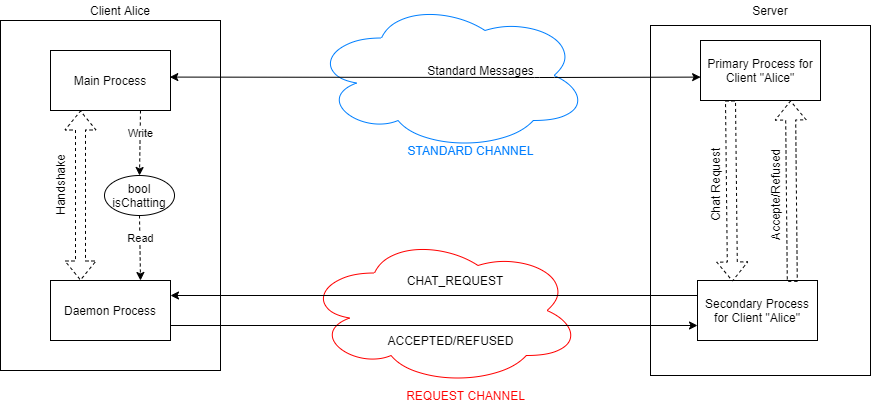
\includegraphics[scale=0.5]{img/chatRequestProtocolTwoProcesses.png}
%		\caption{Solution with two processes}
%		\label {img: chatRequestProtocolTwoProcesses}
%	\end{figure}

%\noindent Notes:


\end{document}          
